\documentclass[10pt,a4paper]{exam}
\usepackage[utf8]{inputenc}
\usepackage{amsmath}
\usepackage{amsfonts}
\usepackage{bbm}
\usepackage{amssymb}
\usepackage{booktabs}
\usepackage{blkarray}
\usepackage{mathdots}
\usepackage{commath}
\usepackage{systeme}
\usepackage{graphicx}
\usepackage[left=.75in,right=.75in,top=.75in,bottom=.75in]{geometry}

\usepackage{tikz}
\usetikzlibrary{chains}



\author{Ryan Honea}
\title{DTMC Problems for Solution}
\begin{document}
\maketitle

\printanswers

\begin{questions}
\question \begin{parts}
\part Draw a transition probability diagram for a DTMC with period 2, but such that $p_{ii}^{(2)} = 1$ for each $i \in S$.

\begin{solution}
\begin{center}
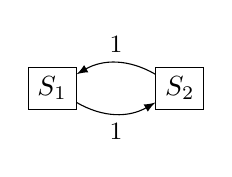
\begin{tikzpicture}[
mynode/.style={
  draw,
  minimum size=1em
  },
every loop/.append style={-latex},  
start chain=going right  
]
\foreach \Value in {1,2}
  \node[mynode,on chain] (s\Value) {$S_{\Value}$};
\path[-latex]
  (s2) edge[bend right] node[auto,swap,font=\small] {$1$} (s1)
  (s1) edge[bend right] node[auto,swap,font=\small] {$1$} (s2);
\end{tikzpicture}
\end{center}
\end{solution}

\part Draw a transition probability diagram for a DTMC with period 2, but such that $p_{ii}^{(2)} \neq 1$ for each $i \in S$.

\begin{solution}
\begin{center}
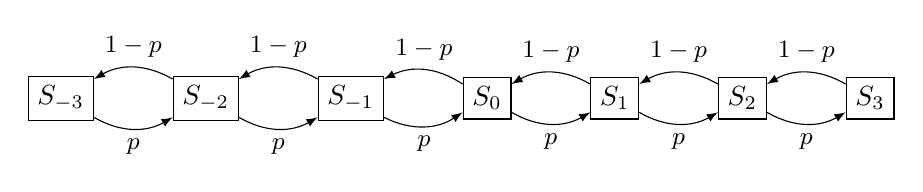
\begin{tikzpicture}[
mynode/.style={
  draw,
  minimum size=1em
  },
every loop/.append style={-latex},  
start chain=going right  
]
\foreach \Value in {-3,...,3}
  \node[mynode,on chain] (s\Value) {$S_{\Value}$};
\path[-latex]
  (s-3) edge[bend right] node[auto,swap,font=\small] {$p$} (s-2)
  (s-2) edge[bend right] node[auto,swap,font=\small] {$p$} (s-1)
  (s-1) edge[bend right] node[below,swap,font=\small] {$p$} (s0)
  (s0) edge[bend right] node[auto,swap,font=\small] {$p$} (s1)
  (s1) edge[bend right] node[auto,swap,font=\small] {$p$} (s2)
  (s2) edge[bend right] node[auto,swap,font=\small] {$p$} (s3)
  (s3) edge[bend right] node[auto,swap,font=\small] {$1-p$} (s2)
  (s2) edge[bend right] node[auto,swap,font=\small] {$1-p$} (s1)
  (s1) edge[bend right] node[auto,swap,font=\small] {$1-p$} (s0)
  (s0) edge[bend right] node[above,swap,font=\small] {$1-p$} (s-1)
  (s-1) edge[bend right] node[auto,swap,font=\small] {$1-p$} (s-2)
  (s-2) edge[bend right] node[auto,swap,font=\small] {$1-p$} (s-3);
\end{tikzpicture}\end{center}

Assume this transition matrix goes from $-\infty$ to $+\infty$ where this is only a zoomed in state space from $-3$ to $+3$. The transitions always follow the form
\begin{align*}
p_{i, i+1} &= p\\
p_{i,i-1} &= 1-p\\
\end{align*}
\end{solution}

\part Draw a transition probability diagram for a DTMC with period 3, but such that $p_{ii}^{(3)} = 1$ for each $i \in S$.

\begin{solution}
\begin{center}
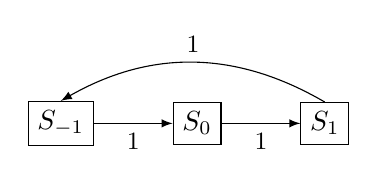
\begin{tikzpicture}[
mynode/.style={
  draw,
  minimum size=1em
  },
every loop/.append style={-latex},  
start chain=going right  
]
\foreach \Value in {-1,...,1}
  \node[mynode,on chain] (s\Value) {$S_{\Value}$};
\path[-latex]
	(s-1) edge node[auto,swap,font=\small] {$1$} (s0)
	(s0) edge node[auto,swap,font=\small] {$1$} (s1)
	(s1.north) edge[bend right] node[auto,swap,font=\small] {$1$} (s-1.north);
\end{tikzpicture}
\end{center}
\end{solution}

\part Draw a transition probability diagram for a DTMC with period 3, but such that $0 < p_{ii}^{(3)} < 1$ for at least one $i \in S$.

\begin{solution}
\begin{center}
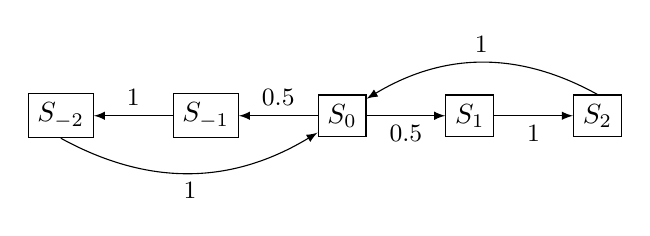
\begin{tikzpicture}[
mynode/.style={
  draw,
  minimum size=1em
  },
every loop/.append style={-latex},  
start chain=going right  
]
\foreach \Value in {-2,...,2}
  \node[mynode,on chain] (s\Value) {$S_{\Value}$};
\path[-latex]
	(s0) edge node[auto,swap,font=\small] {$0.5$} (s1)
	(s0) edge node[auto,swap,font=\small] {$0.5$} (s-1)
	(s-1) edge node[auto,swap,font=\small] {$1$} (s-2)
	(s1) edge node[auto,swap,font=\small] {$1$} (s2)
	(s2.north) edge[bend right] node[auto,swap,font=\small] {$1$} (s0)
	(s-2.south) edge[bend right] node[auto,swap,font=\small] {$1$} (s0);
\end{tikzpicture}
\end{center}
\end{solution}
\pagebreak

\part Draw a transition probability diagram for a DTMC with period 4.

\begin{solution}
\begin{center}
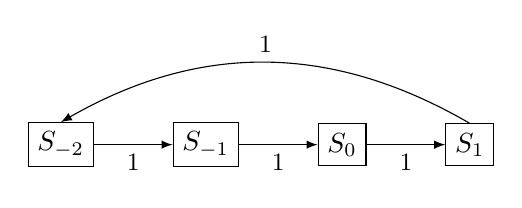
\begin{tikzpicture}[
mynode/.style={
  draw,
  minimum size=1em
  },
every loop/.append style={-latex},  
start chain=going right  
]
\foreach \Value in {-2,...,1}
  \node[mynode,on chain] (s\Value) {$S_{\Value}$};
\path[-latex]
	(s-2) edge node[auto,swap,font=\small] {$1$} (s-1)
	(s-1) edge node[auto,swap,font=\small] {$1$} (s0)
	(s0) edge node[auto,swap,font=\small] {$1$} (s1)
	(s1.north) edge[bend right] node[auto,swap,font=\small] {$1$} (s-2.north);
\end{tikzpicture}
\end{center}
\end{solution}
\end{parts}


\question Draw state diagrams corresponding to each of the following transition probability matrices. For each, specify the classes and state whether each class is transient or recurrent, and state the period. Also, find the stationary \textit{and} limiting distributions (if they exist) for each. If they do not exist, explain why.

$$P_1 = \begin{bmatrix}
2/3 & 1/3 & 0\\1/3 & 0 & 2/3\\0 & 1/3 & 2/3
\end{bmatrix} \quad P_2 = \begin{bmatrix}
0 & 0 & 1 & 0\\.5 & 0 & 0 & .5\\ 0 & 1 & 0 & 0\\0 & 0 & 1 & 0
\end{bmatrix} \quad P_3 = \begin{bmatrix}
1/3 & 2/3 & 0 & 0 & 0\\2/3 & 1/3 & 0 & 0 & 0\\0 & 0 & .5 & .5 & 0\\0 & 0 & .2 & .8 & 0\\0 & 0 & .5 & .5 & 0
\end{bmatrix}$$

\begin{solution}
We will begin with $P_1$ where $P_{1,i}$ is the $i$th node of $P_1$.

\begin{center}
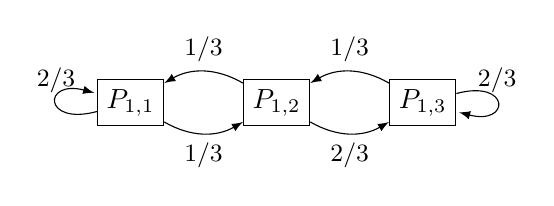
\begin{tikzpicture}[
mynode/.style={
  draw,
  minimum size=1em
  },
every loop/.append style={-latex},  
start chain=going right  
]
\foreach \Value in {1,...,3}
  \node[mynode,on chain] (p\Value) {$P_{1,\Value}$};
\path[-latex]
	(p1) edge[loop left]  node[above,swap,font=\small] {$2/3$} (p1)
	(p1) edge[bend right]  node[auto,swap,font=\small] {$1/3$} (p2)
	(p2) edge[bend right]  node[auto,swap,font=\small] {$1/3$} (p1)
	(p2) edge[bend right] node[auto,swap,font=\small] {$2/3$} (p3)
	(p3) edge[bend right] node[auto,swap,font=\small] {$1/3$} (p2)
	(p3) edge[loop right] node[above,swap,font=\small] {$2/3$} (p3);
\end{tikzpicture}
\end{center}

All states can communicate with one another, so there exists one class composed of $\{P_{1,1}, P_{1,2}, P_{1,3}\}$ which is a recurrent class. Due to the ability of $P_{1,1}$ and $P_{1,3}$ to loop around to each other, the DTMC is aperiodic. 

We can find the stationary distribution by solving the following system.\\
$$\begin{cases}
2/3 \pi_1 + 1/3 \pi_2 = \pi_1\\
1/3 \pi_1 + 1/3 \pi_3 = \pi_2\\
\pi_1 + \pi_2 + \pi_3 = 1
\end{cases} \quad \text{or} \quad \begin{bmatrix}
-1/3 & 1/3 & 0 & 0\\
1/3 & -1 & 1/3 & 0\\
1 & 1 & 1 & 1
\end{bmatrix}$$

which results in $\pi = \begin{bmatrix} 1/4 & 1/4 & 1/2 \end{bmatrix}$. 

This is verified as the limiting distribution by raising the initial matrix to the 100th power (which is reasonably large) which means that not only is the above the stationary distribution, it is the unique stationary distribution.

Now, we analyze $P_{2}$ where $P_{2,i}$ is the $i$th node of $P_2$.

\begin{center}
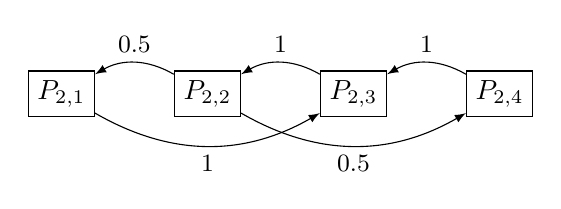
\begin{tikzpicture}[
mynode/.style={
  draw,
  minimum size=1em
  },
every loop/.append style={-latex},  
start chain=going right  
]
\foreach \Value in {1,...,4}
  \node[mynode,on chain] (p\Value) {$P_{2,\Value}$};
\path[-latex]
	(p1) edge[bend right]  node[auto,swap,font=\small] {$1$} (p3)
	(p2) edge[bend right] node[auto,swap,font=\small] {$0.5$} (p1)
	(p2) edge[bend right] node[auto,swap,font=\small] {$0.5$} (p4)
	(p3) edge[bend right] node[auto,swap,font=\small] {$1$} (p2)
	(p4) edge[bend right] node[auto,swap,font=\small] {$1$} (p3);
\end{tikzpicture}
\end{center}

All states can communicate with another, so there exists one class composed of $\{P_{2,1}, P_{2,2}, P_{2,3}, P_{4,3}\}$ which is a recurrent class and has a period of 3.

We find the stationary distribution with the following system

$$\begin{cases} .5\pi_2 = \pi_1\\ \pi_3 = \pi_2 \\ \pi_1 + \pi_4 = \pi_3\\ \pi_1 + \pi_2 + \pi_3 + \pi_4 = 1 \end{cases} \quad \text{or} \quad
\begin{bmatrix}
-1 & .5 & 0 & 0 & 0\\
0 & -1 & 1 & 0 & 0\\
1 & 0 & -1 & 1 & 0\\
1 & 1 & 1 & 1 & 1
\end{bmatrix}$$

This results in a stationary distribution $\pi = \begin{bmatrix}1/6 & 1/3 & 1/3 & 1/6 \end{bmatrix}$. This however is not the limiting distribution, as none exists because this DTMC is periodic.

Now, we analyze $P_3$ where $P_{3,i}$ is the $i$th node of $P_3$.

\begin{center}
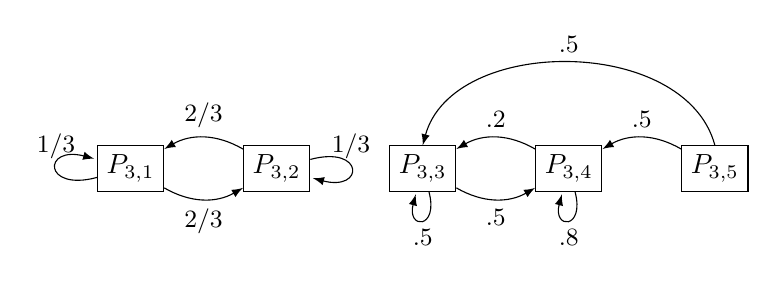
\begin{tikzpicture}[
mynode/.style={
  draw,
  minimum size=1em
  },
every loop/.append style={-latex},  
start chain=going right  
]
\foreach \Value in {1,...,5}
  \node[mynode,on chain] (p\Value) {$P_{3,\Value}$};
\path[-latex]
	(p1) edge[loop left] node[above,swap,font=\small] {$1/3$} (p1)
	(p1) edge[bend right] node[auto,swap,font=\small] {$2/3$} (p2)
	(p2) edge[bend right] node[auto,swap,font=\small] {$2/3$} (p1)
	(p2) edge[loop right] node[above,swap,font=\small] {$1/3$} (p2)
	(p3) edge[loop below] node[below,swap,font=\small] {$.5$} (p3)
	(p3) edge[bend right] node[auto,swap,font=\small] {$.5$} (p4)
	(p4) edge[loop below] node[below,swap,font=\small] {$.8$} (p4)
	(p4) edge[bend right] node[auto,swap,font=\small] {$.2$} (p3)
	(p5) edge[bend right] node[auto,swap,font=\small] {$.5$} (p4)
	(p5.north) edge[bend right = 75, min distance = 1cm] node[auto,swap,font=\small] {$.5$} (p3.north);
\end{tikzpicture}
\end{center}

There are three classes within this DTMC. The classes are $\{P_{3,1}, P_{3,2}\}$, $\{P_{3,3},P_{3,4}\}$, and $\{P_{3,5}\}$. The class $\{P_{3,1}, P_{3,2}\}$ is recurrent and aperiodic, $\{P_{3,3},P_{3,4}\}$ is recurrent and aperiodic, and $\{P_{3,5}\}$ is transient and aperiodic because there is no way to reach the state after leaving it. 

To find the stationary distribution we must solve the following system.

$$\begin{cases}
1/3\pi_1 + 2/3\pi_2 = \pi_1\\ 2/3\pi_1 + 1/3\pi_2 = \pi_2\\ .5\pi_3 + .2\pi_4 + .5\pi_5 = \pi_3 \\ .5 \pi_3 + .8\pi_4 + .5\pi_5 = \pi_4 \\ \pi_1 + \pi_2 + \pi_3 + \pi_4 + \pi_5 = 1
\end{cases} \quad \text{or} \quad \begin{bmatrix}
-2/3 & 2/3 & 0 & 0 & 0 & 0\\
2/3 & -2/3 & 0 & 0 & 0 & 0\\
0 & 0 & -.5 & .2 & .5 & 0\\
0 & 0 & .5 & -.2 & .5 & 0\\
1 & 1 & 1 & 1 & 1 & 1
\end{bmatrix}$$

The stationary distribution follows the form below. It is clear that there is no limiting probability, because the stationary distribution below is not unique (indeed, it shows that there are infinitely many stationary distributions).
$$\begin{bmatrix}
.5 - .7\pi_4\\
.5 - .7\pi_4\\
.4\pi_4\\
\pi_4\\
0
\end{bmatrix}$$.

The above being said, if one were to break down the DTMC into two different Markov Chains comprised of $\{P_{3,1}, P_{3,2}\}$ and $\{P_{3,3}, P_{3,4}, P_{3,5}\}$ the stationary distributions would be the following
$$\begin{bmatrix}
.5 & .5
\end{bmatrix} \quad \text{and} \quad \begin{bmatrix}.29 & .71 & 0\end{bmatrix}$$
which are also the limiting distributions.

\end{solution}

\question The transition probability matrix $P$ is \underline{doubly stochastic} if both $P$ and $P^T$ are stochastic matrices. That is, elements in each row of $P$ sum to 1, and the elements in each column of $P$ sum to 1. Show that if $P$ is doubly stochastic and describes transitions for an irreducible, aperiodic DTMC with $M$ states, then the limiting probabilities for the two DTMCs described by $P$ and $P^T$ are the same and are given by 
$$\pi_i = \frac{1}{M} \quad \text{for each } i.$$

\begin{solution}
We will show that the stationary distribution where $\pi_i = \frac{1}{M}$ is the unique stationary distribution and thus is the limiting distribution. 

Because $P$ is irreducible, all states are recurrent, and by Theorem 4.1 in the text, the DTMC is ergodic. Therefore, $\lim_{n \to \infty} P_{ij}^{(n)}$ exists, and $\pi_j = \lim_{n \to \infty} P_{ij}^{(n)}$ is the unique stationary distribution.

Now, letting $\pi_i = \frac{1}{M}$, we have

$$\pi_j = \sum_{i=1}^M  \frac{1}{M} P_{ij} = \frac{1}{M}\sum_{i=1}^M P_{ij}$$

Note that due to the doubly stochastic nature of $P$, $\sum_{i = 1}^M P_{ij} = 1$, so we have
$$\pi_j = \frac{1}{M}$$ This also satisfies the condition that $\sum_{i=1}^M \pi_i =1$ because $M * \frac{1}{M} = 1$. Therefore $\pi_i = \frac{1}{M}$ is the unique stationary distribution.

A similar argument can be made for $P^T$ as the column sum of $P_T$ will also be 1 by the doubly stochastic nature, and therefore by the logic before, it will also have limiting distribution $\pi_i = \frac{1}{M}$
\end{solution}


\question Consider the random walk on the integers $\{...,-2,-1,0,1,2,...\}$ with transition probabilities $p_{i,i+1} = p =  1 - p_{i,i-1}$ for all $i \in \mathbb{Z}$. Use the strong law of large numbers to give another proof that the Markov chain is transient when $p \neq 1/2$. \textit{Hint: Can you argue that as $n \rightarrow \infty$ the state at time $n$ represented as $\sum_{i=1}^nY_i$ (the sum of individual moves) tends to infinity if $p > 1/2$ and so the initial state is visited a finite numbers of times with probability 1?}

\begin{solution}
We will define a random variable $Y_i$ where $$Y_i = \begin{cases}1, & \text{when } X_i > X_{i-1}\\
-1, &\text{when }  X_i < X_{i-1}\end{cases}$$ where $X_i$ is the state at time $i$.

Therefore, this is a bernoulli random variable where $E[Y_i] = p*1 + (1-p)*-1 = 2p - 1$. It is clear that when $p > 0.5$, then $E[Y_i] > 0$ and when $p < 0.5$, then $E[Y_i] < 0$.

By the strong law of large numbers,

$$\frac{1}{n} \sum_{i=1}^n Y_i = E[Y_i] \quad \text{as} \quad n \to \infty$$

Therefore, it is clear that when $p \neq 0$, then $$\lim_{n\to\infty}\sum_{i=1}^n Y_i = \begin{cases}\infty & \text{when } p > .5\\-\infty & \text{when } p < .5\end{cases}$$

Therefore the initial states are only limited a finite amount of times with probability 1.
\end{solution}

\pagebreak

\question A DNA nucleotide takes one of four letters (A, D, C, G). We can model nucleotide mutation with a discrete-time Markov chain in the following way. Assume the probability that a nucleotide at a particular location changes with probability $3\alpha$, and that conditioned that there is indeed a change, then it is equally likely to change to any of the three other letters. Here, $\alpha$ is some constant in $(0, 1/3)$.

\begin{parts}
\part Show $p_{1,1}^{(n)} = .25 + .75(1-4\alpha)^n$.
\begin{solution}
We will prove this by induction.
\begin{align*}
p_{1,1}^{(0)}  &= .25 + .75(1-4\alpha)^0\\
					&= 1\\
p_{1,1}^{(1)} 	&= 1 - 3\alpha\\
					&= .25 + .75 + 3\alpha\\
					&= .25 + .75(1-4\alpha)^1\\
\end{align*}

So the trivial cases are shown. Now, we assume $$p_{1,1}^{(k)} = .25 + .75(1-4\alpha)^k$$
and show that
$$p_{1,1}^{(k+1)} = .25 + .75(1-4\alpha)^{k+1}$$

By the law of total probability, we have the following

\begin{align*}
p_{1,1}^{(k+1)} 	&= p_{1,1}^{(k)}p_{1,1}^{(1)} + p_{1,2}^{(k)}p_{2,1}^{(1)} + p_{1,3}^{(k)}p_{3,1}^{(1)} + p_{1,4}^{(k)}p_{4,1}^{(1)} & \text{(Law of Total Probability)}\\
						&=p_{1,1}^{(k)}(1 - 3\alpha) + \alpha(p_{1,2}^{(k)}+p_{1,3}^{(k)}+p_{1,4}^{(k)})\\
						&= p_{1,1}^{(k)}(1 - 3\alpha) + \alpha(1 - p_{1,1}^{(k)}) & \text{(As row sum must equal 1)}\\
						&= \alpha + p_{1,1}^{(k)} - 4\alpha p_{1,1}^{(k)}\\
						&=\alpha + p_{1,1}^{(k)}(1-4\alpha)\\
						&=\alpha + .25(1-4\alpha) + .75(1-4\alpha)^k(1-4\alpha)\\
						&=.25 + .75(1-4\alpha)^{k+1} = p_{1,1}^{k+1}
\end{align*}
\end{solution}
\part What is the long-run proportion of time the DTMC is in each state?
\begin{solution}
The transition matrix is
$$P = \begin{bmatrix}
1 - 3\alpha & \alpha & \alpha & \alpha\\
\alpha & 1 - 3\alpha & \alpha & \alpha\\
\alpha & \alpha & 1 - 3\alpha & \alpha\\
\alpha & \alpha & \alpha & 1 - 3\alpha
\end{bmatrix}$$
which is doubly stochastic. We previously proved that the limiting distribution $\pi_i = 1/M$ for an irreducible recurrent matrix. So, if we have $$
\pi = \begin{bmatrix}
1/4 & 1/4 & 1/4 & 1/4\\
\end{bmatrix}
$$
\end{solution}
\end{parts}

\pagebreak

\question Every morning Boosty goes to work he is just as likely to leave through the front door as he is the back door. When he leaves, he chooses a random pair of sunglasses by the door from which he leaves (or goes without them if there are none by that door). When he returns, he is equally likely to enter through the front door as he is through the back, and he leaves his sunglasses by that door. if he owns $m$ pairs of sunglasses, what proportion of time does he go without wearing them?

\begin{solution}
Consider the random variable $X_t$ that describes the number of sunglasses at the front door. There are four cases that can occur with equal probability, enter and leave the front door, enter and leave the back door, enter front leave back, enter back leave front. This gives the following
$$X_{t+1} = \begin{cases}
X_t + 1, & \text{if leaving back and entering front \& } X_t \neq m\\
X_t - 1, & \text{if leaving fron and entering back \& } X_t \neq 0\\
X_t, & o/w
\end{cases}$$

For example, this would result in the following transition matrix for $m = 5$.

$$\begin{blockarray}{ccccccc}
& 0 & 1 & 2 & 3 & 4 & 5\\
\begin{block}{c[cccccc]}
0 & .75 & .25 & 0 & 0 & 0 & 0\\
1 & .25 & .75 & .25 & 0 & 0 & 0\\
2 & 0 & .25 & .50 & .25 & 0 & 0\\
3 & 0 & 0 & .25 & .50 & .25 & 0\\
4 & 0 & 0 & 0  & .25 & .50 & .75\\
5 & 0 & 0 & 0 & 0 & .25 & .75\\
\end{block}
\end{blockarray}$$

It's immediately clear that this is a doubly stochastic matrix for any $m$ and so with $m+1$ states, the stationary distribution for all $\pi_j = \dfrac{1}{m+1}$. From this we can solve the problem.

\begin{align*}
P(\text{Leave w/o Sunglasses}) &= P(\text{Exit Front}\cap X_t = 0) + P(\text{Exit Back}\cap X_t = m)\\
												&= P(\text{Exit Front})P(X_t = 0) + P(\text{Exit Back})P(X_t = m)\\
												&= \frac{1}{2}\frac{1}{m+1} + \frac{1}{2}\frac{1}{m+1}\\
												&= \frac{1}{m+1}
\end{align*}
\end{solution}
\pagebreak
\question Every day Mustang Sally receives a speeding ticket, she receives another one on the following day with probability 0.1. Every day she doesn't receive a ticket, she receives one the following day with probability 0.5. Each day she does not receive a ticket she goes to dinner with Otis with probability 0.8 and dines alone otherwise alone. Each day she receives a ticket, she goes to dinner with Marvin with probability 0.4, and otherwise alone. What proportion of time does she have dinner with Otis? with Marvin? alone?

\begin{solution}
We will denote speeding and eating with Marvin as $p_{s,m}$, speeding and eating alone as $p_{s,a}$, not speeding and eating with Otis as $p_{n,o}$, and not speeding and eating alone as $p_{n,a}$. 

This creates the following transition matrix.

\[
\begin{blockarray}{ccccc}
& s,m & s,a & n,o & n,a \\
\begin{block}{c[cccc]}
s,m & (.1)(0.4) & (.1)(0.6) & (.9)(.8) & (.9)(.2)\\
s,a  & (.1)(0.4) & (.1(0.6) & (.9)(.8) & (.9)(.2)\\
n,o  & (.5)(0.4) & (.5)(0.6) & (.5)(0.8) & (.5)(0.2)\\
n,a  & (.5)(0.4) & (.5)(0.6) & (.5)(0.8) & (.5)(0.2)\\
\end{block}
\end{blockarray} = \begin{blockarray}{ccccc}
& s,m & s,a & n,o & n,a \\
\begin{block}{c[cccc]}
s,m & .04 & .06 & .72 & .18\\
s,a  & .04 & .06 & .72 & .18\\
n,o  & .2 & .3 & .4 & .1\\
n,a  & .2 & .3 & .4 & .1\\
\end{block}
\end{blockarray}
\]

We can find the limiting probability by exponentiating the matrix to a significantly large power which gives us the proportions of time. This is done in Octave with the following code.
\begin{verbatim}
P = [.04 .06 .72 .18;
> .04 .06 .72 .18;
> .2 .3 .4 .1;
> .2 .3 .4 .1];
P^1000
\end{verbatim}

This results in the following:'
$$\begin{blockarray}{ccccc}
& s,m & s,a & n,o & n,a \\
\begin{block}{c[cccc]}
s,m & .143 & .214 & .514 & .129\\
s,a  & .143 & .214 & .514 & .129\\
n,o  & .143 & .214 & .514 & .129\\
n,a  & .143 & .214 & .514 & .129\\
\end{block}
\end{blockarray}$$

So, she spends her time with Marvin 14.3\% of the time, with Otis 51.4\% of the time, and herself 34.3\% of the time.

\end{solution}

\question The ACME Actuarial Group employs a large number of employees (there are $N$ of them). At any time, each employee holds one of three ranks: $I$, $II$, or $III$. Each employee independently changes job classification according to a DTMC with transition probability matrix

$$P = \begin{blockarray}{cccc}
& I & II & III\\
\begin{block}{c(ccc)}
I & .6 & .3 & .1\\
II & .5 & .2 & .3\\
III & .1 & .5 & .4\\
\end{block}
\end{blockarray}$$
In the long-run, what percentage of employees are in each classification?

\begin{solution}
The limiting and stationary distribution of $P$ is
$$\begin{bmatrix}
.45 & .32 & .23
\end{bmatrix}$$
(found in Octave with similar code to P7.)

Therefore, the times spent on average in each state are 45\% in state I, 32\% in state II, and 23\% in state III.
\end{solution}

\pagebreak

\question Let $\pi_i$ denote the long-run proportion of time a given irreducible DTMC is in state $i$.
\begin{parts}
\part Why must $\pi_i$ also equal the proportion of transitions that are into state $i$, as well as the proportion of transitions that are made out of state $i$?
\begin{solution}
If something enters into state $i$, given that it is not absorbing, it must therefore transition out of state $i$. It is clear that if $\pi_i$ represents the amount of time state $i$ is entered, it must equivalently leave state $i$ as much as it is entered. It wouldn't make sense to say that one enters a grocery store five times and leaves it 3 times. It also wouldn't make sense to say one has entered the grocery store 4 times but been there 5 times. So the statements are all essentially equivalent over an infinite period of time.
\end{solution}
\part $\pi_ip_{ij}$ represents the proportion of transitions that are of what type?
\begin{solution}
It represents the proportion of transitions that start in $i$ and enter $j$.
\end{solution}
\part $\sum_i\pi_ip_{ij}$ represents the proportion of transitions that are of what type?
\begin{solution}
It represents the proportion of transitions that enter $j$. Specifically, it is the sum of transitions that start in $i$ and enter $j$ over the $i$s.
\end{solution}
\part Explain why 
$$\pi_j = \sum_i \pi_ip_{ij}$$
\begin{solution}
Based on part (a), we can see that one enters and exits state $j$ with equal proportion and is thus in state $j$ with equal proportion. So, if $\sum_i \pi_ip_{ij}$ represents the amount of time that one transitions into $j$ by the results from (c), then by the results of $(a)$, we have the above formula.
\end{solution}
\end{parts}






\question Let $A$ be a subset of the state space for a DTMC.
\begin{parts}
\part Explain the meaning of
$$ \sum_{i \in A} \sum_{j \in A^c} \pi_i p_{ij} $$
\begin{solution}
This is the probability that one transitions from a state within $A$ to a state outside of $A$ (or in $A^c$).
\end{solution}
\part Explain the meaning of
$$ \sum_{i \in A^c} \sum_{j \in A} \pi_i p_{ij} $$
\begin{solution}
This is the probability that one transitions from a state outside of $A$ (or in $A^c$) into a state within $A$.
\end{solution}
\part Explain why the two quantities above are equal.
\begin{solution}
Similar to the logic within problem 9, if $A$ is entered some percent of the time, it must also be left the same percent of the time. That is, they both represent the amount of time spent within $A$. 
\end{solution}
\end{parts}






\pagebreak


\question Gene Kelly has $k$ umbrellas he uses to keep him dry on his way to and from work. If he is at home at the beginning of a rainy date, he will take an umbrella to work (provided there is one at home). If it is raining when he leaves work, he will take an umbrella home (provided there is one at work). He doesn't take an umbrella if it is not rainy. Suppose the chance of rain is always $p$.

\begin{parts}
\part Define a Markov chain with $K + 1$ states that will help determine the proportion of time Gene gets wet.
\begin{solution}
We define a random variable $X_t = $\# of Umbrellas at Current Location.
Starting with the first case, if we have 0 umbrellas at home and $k$ umbrellas at work, that means that all umbrellas are at the workplace with probability 1..
If we have 1 umbrella at home and $k-1$ umbrellas at work then it didn't rain, but if we have $k$ umbrellas at work, then it did rain.
This continues to if we have $k$ umbrellas at work, then we can have $0$ at work if it did not rain and $1$ if it did rain with probability $p$. So, we have the following system
$$\begin{cases}
p_{i, r - i} = 1 - p\\
p_{i, r - i + 1} = p\\
p_{0, k} = 1\\
0, \quad  o/w\end{cases}
$$
An example matrix for K = 3 would be

$$P = \begin{blockarray}{ccccc}
& 0 & 1 & 2 & 3\\
\begin{block}{c[cccc]}
0 & 0 & 0 & 0 & 1\\
1 & 0 & 0 & 1-p & p\\
2 & 0 & 1-p & p & 0\\
3 & 1 - p & p & 0 & 0\\
\end{block}
\end{blockarray}$$


\end{solution}
\part Find the limiting probabilities.
\begin{solution}
We know that because this DTMC is an irreducible recurrent matrix, we know that the stationary distribution is the limiting distribution. So, we can solve the following system of equations.
\begin{align*}
\pi_0 &= (1-p)\pi_k\\
\pi_k &= \pi_0 + p\pi_1\\
\implies \pi_0 &= (1-p)(\pi_0 + p\pi_1)\\
					&= (1-p)\pi_0 + (1-p)p\pi_1\\
					&= (1-p)\pi_1
\end{align*}
The above implies that $\pi_k = \pi_1$ and the same logic can be applied to show that $\pi_i = \pi_j \forall i, j \in 1...k$.

So, we also have
$$\sum \pi_k = 1$$
and therefore
\begin{align*}
\pi_0 + K\pi_k 	&= 1\\
(1-p)\pi_k + K \pi_k &= 1\\
\pi_k &= (1 - p + K)^{-1}\\
pi_1 &= (1 - p)(1 - p + K)^{-1}\\
\end{align*}

So the limiting distribution is
$$\pi_i = \begin{cases}
\dfrac{1-p}{1 - p + K}, & i = 0\\
\dfrac{1}{1 - p + K}, & i = 1...K\\
0, & o/w
\end{cases}$$
\end{solution}
\part What fraction of the trips does Gene get wet?
\begin{solution}
We are interested in the case where there are 0 umbrellas in your location and it is raining, or $p\pi_0$. So the fraction of the time is
$$p\pi_0 = \frac{p(1-p)}{1 - p + K}$$
\end{solution}

\part When $K = 3$, what value of $p$ maximizes the fraction of time Gene gets wet?
\begin{solution}
We utilize the ratio found above and solve for $p$ when $$\frac{\dif}{\dif p} \frac{p(1-p)}{1-p+3} = 0$$
So, we have

\begin{align*}
0	&=\frac{\dif}{\dif p} \frac{p(1-p)}{1-p+3}\\
	&= \frac{p^2 - 8p + 4}{(p-4)^2}\\
	&= p^2 - 8p + 4\\
p	&= 2(2 \pm \sqrt{3})
\end{align*}
\end{solution}
\end{parts}











\question If you repeatedly roll a fair die, what is the expected number of rolls required until you see
\begin{parts}
\part 1, 2, 3, 4, 5, 6?
\begin{solution}
This is just $[(1/6)^6]^{-1} = 46,656$
\end{solution}
\part 6, 6, 6?
\begin{solution}
$$\left(\frac{1}{6}\right)^{-1} + \left(\frac{1}{6^2}\right)^{-1} + \left(\frac{1}{6^3}\right)^{-1} = 258$$
\end{solution}
\part 3, 6, 2, 4, 3, 6?
\begin{solution}
$$\left(\frac{1}{6^6}\right)^{-1} + \left(\frac{1}{6^2}\right)^{-1} = 46692$$
\end{solution}
\part Can you explain why the mean time to see ``362436" for the first time is more than the mean time to see ``123456" for the first time?
\begin{solution}
The mean time for ``362436" includes the observation of a repeated pattern (36) while ``123456" contains no pattern. So, for the first case, you have to calculate the expected number of rolls to find ``362436" plus the expected time between the pattern ``36."
\end{solution}
\end{parts}









\pagebreak
\question $M$ balls are distributed into two urns. Every second, one ball is chosen uniformly at random and moved to the other urn. Let $X_n$ denote the number of balls in urn \# 1 just after the $n$th move. Show that
\begin{parts}
\part $E[X_{n+1}] = 1 + (1 - 2/M)E[X_n]$.
\begin{solution}
Note the below probabilities that give us our Markov Chain, 
$$p_{0,1} = 1$$
$$p_{M, M-1} = 1$$
$$p_{i, i - 1} = \frac{i}{M}$$
$$p_{i, i + 1} = \frac{M - i}{M}$$
Combining all of these probabilities, we get the following
\begin{align*}
E[X_{n+1}] 	&= E[X_n] + (-1)\frac{E[X_n]}{M} + (+1)\frac{M-E[X_n]}{M}\\
					&= E[X_n] + \frac{M - 2E[X_n]}{M}\\
					&=  E[X_n] + 1 - \frac{2}{M}E[X_n]\\
					&= 1 + \left(1 - \frac{2}{M}\right)E[X_n]
\end{align*}
\end{solution}
\part $E[X_n] = M/2 + \left(\frac{M-2}{M}\right)^n (E[X_0] - M/2)$
\begin{solution}
\begin{align*}
E[X_n]	&= 1 + \left(1 - \frac{2}{M}\right)E[X_{n-1}]\\
			&= 1 + \left(\frac{M-2}{M}\right)E[X_{n-1}]\\
			&= 1 + \left(\frac{M-2}{M}\right)\left[1 + \left(\frac{M-2}{M}\right)E[X_{n-2}]\right]\\
			&= 1 + \frac{M-2}{M} + \left(\frac{M-2}{M}\right)^2E[X_{n-2}]\\
			&= \sum_{i=0}^{n-1} \left(\frac{M-2}{M}\right)^i + \left(\frac{M-2}{M}\right)^n E[X_0]\\
			&= \sum_{i=0}^{n} \left(\frac{M-2}{M}\right)^i - \left(\frac{M-2}{M}\right)^n +  \left(\frac{M-2}{M}\right)^n E[X_0]\\
			&= \sum_{i=0}^{\infty} \left(\frac{M-2}{M}\right)^i - \sum_{i=n}^{\infty} \left(\frac{M-2}{M}\right)^i +  \left(\frac{M-2}{M}\right)^n E[X_0]\\
			&= \frac{M}{2} - \left(\frac{M-2}{M}\right)^n\sum_{i=0}^{\infty} \left(\frac{M-2}{M}\right)^i+  \left(\frac{M-2}{M}\right)^n E[X_0]\\
			&= \frac{M}{2} - \left(\frac{M-2}{M}\right)^n\frac{M}{2}+  \left(\frac{M-2}{M}\right)^n E[X_0]\\
			&= \frac{M}{2} - \left(\frac{M-2}{M}\right)^n\left(E[X_0] - \frac{M}{2}\right)
\end{align*}
\end{solution}
\end{parts}
\pagebreak
\question In Exercise 8, suppose the three job classifications are $I$, $II$, and $III$ with $p_{I,I} = .6$, etc. Then if an employee begins in classification $I$, what is the expected amount of time spent in each of the three classifications over the first 10 times? Over the first 20 times? Over the first 100 times? What are these expectations divided by the numbers of times converging to?

\begin{solution}
Using the following Octave script with varying numDays, the results are found for 10, 20, and 100.
\begin{verbatim}
P = [.6 .3 .1;.5 .2 .3;.1 .5 .4];
result = eye(3)
numDays = 10;
for i = 2:numDays
    result = result + P^i;
endfor
result
\end{verbatim}

Over the first 10 days, given that one starts in position $I$, they spend 5.3237  in $I$, 2.7848 in $II$, and 1.8916 in $III$. Over the first 20 days, given that one starts in position $I$, they spend 9.8442  in $I$, 5.9354 in $II$, and 4.2203 in $III$. Over the first 100 days, given that one starts in position $I$, they spend 46.009  in $I$, 31.141 in $II$, and 22.850 in $III$.

They are approaching the stationary distribution when divided by the number of times.
\end{solution}

\question Consider a branching process with $\mu < 1$. Show that $X_0 = 1$ implies the expected number of distinct individuals that were ever members of the population is $1/(1-\mu)$. Remember that each population member lives for exactly one discrete time unit, and sort-of dies while giving birth to all of its offspring at the same time.

\begin{solution}
From the notes, we know that $E[X_n] = \mu^n$ given that $X_0= 1.$ To find the total number of distinct individuals that were ever members of the population, we need to find
$$\sum_{i=0}^\infty X_0$$
We know this to be 
$$\sum_{i=0}^\infty \mu^i$$
and if $\mu < 1$, this is a geometric series where the solution is 
$$\dfrac{1}{1-\mu}$$
\end{solution}

\pagebreak









\question In a branching process with $X_0 = 1$ and $\mu > 1$, prove that $\pi_0$ is the smallest positive number that satisfies
$$\pi_0 = \sum_{j=0}^\infty \pi_0^jp_j$$
\begin{solution}
Let $G(\theta)$ be the probability generating function
$$G(\theta) = \sum_{k = 0}^{\infty} p_k\theta^k$$
In this case, we have
$$\pi_0 = P(X_n = 0) = \sum_{k=0}^\infty p_k P(X_{n-1} = 0)^k$$
Also, in the case where $\mu > 1$, we can also observe that $p_k$ is nondecreasing (that is $p_0 \leq p_1 \leq ... \leq p_\infty$).  Since $p_k \leq 1 \forall k$, this implies that $\lim_{n \to \infty} p_n$ exists which is
$p_\infty = G(p_\infty)$ so $p_\infty$ is a solution of $G(x) = x$.

So, let $p$ be the smallest solution of $G(x) = x)$. We will show that this is $p_\infty$. Also note that $G(x)$ is a decreasing function (which is trivially shown). So, by the definition of probability generating functions, we have

$$p_1 = G(p_0) \leq G(p)$$
$$p_2 = G(G(p_0)) \leq G(p)$$
$$p_3 = G(G(G(p_0))) \leq G(p)$$
$$p_n = G_n(p_0) = G(p_{n-1}) \leq G(p)$$
so that $p_n \leq p \forall n$. If we take the limit, it gives that $p_\infty \leq p$, however, as $p$ is the smallest solution to $G(x) = x$, then $p_\infty = p$.
\end{solution}







\pagebreak




\question For a branching process, compute $\pi_0$ when
\begin{parts}
\part $p_0 = .25, p_2 = .75$
\begin{solution}
\begin{align*}
\pi_0 &= .25 + .75\pi_0^2\\
0		&= .25 - \pi_0 + .75\pi_0^2\\
		&= 3\pi_0^2 - 4\pi_0 + 1\\
		&= (x-1/3)(x-1)
\end{align*}
We choose the smallest positive value that satisfies the equation which is $\frac{1}{3}$.
\end{solution}
\part $p_0 = .25, p_1 =.5, p_2 = .25$
\begin{solution}
\begin{align*}
\pi_0 	&= .25 + .5\pi_0 + .25\pi_0^2\\
0			&= .25 - .5\pi_0 + .25\pi_0^2\\
			&= \pi_0^2 - 2\pi_0 + 1\\
			&= (\pi_0 - 1)^2\\
\end{align*}
So $\pi_0 = 1$ and so the population will certainly go extinct.
\end{solution}
\part $p_0 = 1/6, p_1 = .5, p_3 = 1/3$
\begin{solution}
\begin{align*}
\pi_0 &= \frac{1}{6} + .5\pi_0 + \frac{1}{3}\pi_0^3\\
0		&= \frac{1}{6} - .5\pi_0 + \frac{1}{3}\pi_0^3\\
		&= 2\pi_0^3 - 3\pi_0 + 1\\
		&= (x-1)\left(x - \frac{1}{2}(-1 \pm \sqrt{3})\right)
\end{align*}
We take the smallest positive value that satisfies the equation which is $$\pi_0 = \frac{1}{2}(-1 + \sqrt{3})$$
\pagebreak
\end{solution}
\end{parts}
\pagebreak













\question Prove that if you're given an irreducible DTMC with transition probabilities $p_{ij}$, and if you can find positive numbers $\pi_i$, $i \geq 0$ with $\sum_i \pi_i = 1$ and some other transition probability matrix $Q$ so that
$$\pi_i p_{ij} = \pi_j q_{ji}$$
then the $q_{ij}$ are the transition probabilities of the reversed chain and the $\pi_i$ are stationary probabilities for both the original and the reversed chain.

\begin{solution}
If we can show that there exists a solution to $\pi P = \pi$ because the above equation satisfies the time reversible property already. 

We can show that a solution exists by fixing some $j$ and summing over the respective $i$s.

\begin{align*}
\sum_i \pi_i p_{ij} &= \sum_i \pi_jq_{ji}\\
							&= \pi_j \sum_i q_{ji}\\
							&= \pi_j & \text{As Q is a DTMC}
\end{align*}
And so $\pi_i$ is also a solution for the reverse chain as well as the original chain. Note that this only holds true in the case that $q_{ji}$ satisfies the time reversibility requirement.
\end{solution}
















\question $M$ balls are distributed among $m$ urns. Each second, one of the balls is chosen uniformly at random and to one of the other $m - 1$ urns chosen at random. Consider a DTMC whose state space is
$$\left\{ (n_1, n_2, ..., n_m) : \sum_i n_i = M, n_i \in \{0,1,...,M\} \text{ for each } i \right\}$$
Here, $n_i$, is the number of balls in urn \#$i$. Guess the limiting probabilities for this DTMC. Then verify your guess, showing at the same time that this DTMC is time-reversible.

\begin{solution}
In the Markov chain below for $n_1$, I set the number of urns $m$ to be $u$ for sake of readability.
$$n_1 = \begin{blockarray}{cccccccc}
       & 0                   & 1                             & 2                             & 3                             & \dots  & M-1                               & M                          \\
\begin{block}{c[ccccccc]}
0      & \frac{u-2}{u-1} & \frac{1}{u-1}             & 0                         & 0                         &        & 0                             & 0                      \\
1      & \frac{1}{M}     & \frac{(M-1)(u-2)}{M(u-1)} & \frac{M-1}{M(u-1)}        & 0                         &        &                               &                        \\
2      & 0               & \frac{2}{M}               & \frac{(M-2)(u-2)}{M(u-1)} & \frac{M-2}{M(u-1)}        &        &                               &                        \\
3      & 0               & 0                         & \frac{3}{M}               & \frac{(M-3)(u-2)}{M(u-1)} &        &                               &                        \\
\vdots &    \vdots             &                           &                           &                           & \ddots &                               &                        \\
M-1    &   0              &                           &                           &                           &        & \frac{(M-(M-1))(u-2)}{M(u-1)} & \frac{M-(M-1)}{M(u-1)} \\
M      &      0           &                           &                           &                           &        & 1                             & 0                     \\
\end{block}
\end{blockarray} $$

The following definitions make up this Markov Chain
\begin{align*}
p_{i,i-1} &= \frac{i}{M}\\
p_{i,i} &= \frac{(M-i)(u-2)}{M(u-1)}\\
p_{i,i+1} &= \frac{M-i}{M(u-1)}
\end{align*}
which always sum to 1.

I hypothesize that the stationary distribution of $n_1$ is $$\pi_i = \binom{M}{i}\left(\frac{1}{u}\right)^i \left(1-\frac{1}{u}\right)^{M-i} \sim \text{Bin}\left(M, \frac{1}{u}\right)$$ I will verify this for $\pi_1 = \pi_0 p_{0j} + \pi_1 p_{1j} + \pi_2 p_{2j}$ and then discuss why this is true. Note that the full computation of this was done in Mathematica using it's symbolic mathematics features.
\begin{align*}
\sum_{i=1}^{n} \pi_i p_{i1}	&= \binom{M}{0}\left(\frac{1}{u}\right)^0 \left(1 - \frac{1}{u}\right)^{M-0} \left(\frac{1}{u-1}\right)\\
		&+ \binom{M}{1}\left(\frac{1}{u}\right)^1 \left(1 - \frac{1}{u}\right)^{M-1} \left(\frac{(M-1)(u-2)}{M(u-1)}   \right)\\
		&+  \binom{M}{2}\left(\frac{1}{u}\right)^2 \left(1 - \frac{1}{u}\right)^{M-2} \left(\frac{2}{M}\right)\\
		&= \frac{M\left(\frac{u-1}{u}\right)^M}{u-1}\\
		&= \binom{M}{1} \frac{\left(\frac{u-1}{u}\right)^M}{u-1} =\binom{M}{1} \frac{\left(\frac{u-1}{u}\right)^{M-1}}{(u-1)\left(\frac{u}{u-1}\right)}\\
		&= \binom{M}{1}\left(\frac{1}{u}\right)^1 \left(1 - \frac{1}{u}\right)^{M-1} = \pi_1
\end{align*}

This isn't a proper proof, but the thought process behind the stationary distribution is as follows. For any urn $i$, each should have the same stationary distributions like above. For each urn $i$, the amount of balls within it can be considered "successes," which leads to the binomial distribution. Indeed, for $m$ balls, there are $\binom{m}{j}$ ways to distribute the balls in an urn each occurring with probability $u^{-j}\left(1-u^{-1}\right)^{M-j}$.

The time reversible equations say that
$$\pi_ip_{ij} = \pi_jp_{ji} \forall i,j$$
and so we can verify this is time reversible. Note that the only cases that exist are
\begin{align*}
\pi_i p_{i,i+1} &= \pi_{i+1} p_{i+1,i}\\
\pi_i p_{i,i} &= \pi_i p_{i,i}\\
\pi_i p_{i,i-1} &= \pi_{i-1} p_{i-1,i}
\end{align*}
Note that if we set $j = i - 1$, the first and third case are essentially the same and the second is trivial. So, we only need to show that the first is true.

\begin{align*}
\pi_i p_{i,i+1}		&= \binom{M}{i}\left(\frac{1}{u}\right)^i \left(1 - \frac{1}{u}\right)^{M-i} \left( \frac{M-i}{M(u-1)}\right)\\
						&= \frac{M!}{(M-i)!i!} \left(\frac{1}{u}\right)^i \left(\frac{u-1}{u}\right)^{M-i} \left( \frac{M-i}{M(u-1)}\right)\\
						&= \left(\frac{i+1}{M}\right)\frac{M!}{(M-(i+1))!(i+1)!}\left(\frac{1}{u}\right)^i \left(\frac{u-1}{u}\right)^{M}\left(\frac{u}{u-1}\right)^i \left(\frac{1}{u-1}\right)\\
						&= \binom{M}{i+1} \left(\frac{1}{u^M}\right) \left(\frac{(u-1)^M}{(u-1)^{i+1}}\right)\left(\frac{i+1}{M}\right)\\
						&= \binom{M}{i+1} \left(\frac{1}{u^{i+1}u^{M-(i+1)}}\right) \left((u-1)^{M-(i+1)}\right) \left(\frac{i+1}{M}\right)\\
						&= \binom{M}{i+1} \left(\frac{1}{u}\right)^{i+1} \left(1 - \frac{1}{u}\right)^{M-i-1} \left(\frac{i+1}{M}\right)\\
						&= \pi_{i+1} p_{i+1,i}
\end{align*}
Therefore the solution for $\pi$ is correct and this matrix is time reversible.

\textit{Note:} If considering the urns as a whole, one can consider the distribution of the $n_i$s as a whole state space which would be multinomial instead of binomial (i.e)
$$\pi(n_1, n_2, ..., n_u) = \frac{M!}{\prod_{i=1}^n n_i!} \left(\frac{1}{u}\right)^M$$
\end{solution}

\pagebreak

\question A knight begins at the corner of a chessboard and begins to move about the board, making only the legal moves a knight can make. Each move is made uniformly at random among the choices of moves at the time. What is the expected number of moves until it returns to its original position? \textit{Hint: Work through example 4.36 first.}

\begin{solution}
The expected time to return to a location is $\pi_i^{-1}$, and so we must find $\pi_i$. Using the time reversibility equations in Example 4.36 from the text, $\pi_i$ can be found with 
$$\pi_i = \frac{\sum_j w_{ij}}{\sum_i\sum_j w_{ij}}$$
If we can express this graph as a collection of nodes with weights, then we can find the solution. 

Consider the chess board below, where the boxes are each assigned a weight by how many ways a knight can move out of the position.
\begin{center}
\begin{tabular}{rcccccccc}
\cline{2-9}
\multicolumn{1}{r|}{8} & \multicolumn{1}{c|}{2} & \multicolumn{1}{c|}{3} & \multicolumn{1}{c|}{4} & \multicolumn{1}{c|}{4} & \multicolumn{1}{c|}{4} & \multicolumn{1}{c|}{4} & \multicolumn{1}{c|}{3} & \multicolumn{1}{c|}{2} \\ \cline{2-9} 
\multicolumn{1}{r|}{7} & \multicolumn{1}{c|}{3} & \multicolumn{1}{c|}{4} & \multicolumn{1}{c|}{6} & \multicolumn{1}{c|}{6} & \multicolumn{1}{c|}{6} & \multicolumn{1}{c|}{6} & \multicolumn{1}{c|}{4} & \multicolumn{1}{c|}{3} \\ \cline{2-9} 
\multicolumn{1}{r|}{6} & \multicolumn{1}{c|}{4} & \multicolumn{1}{c|}{6} & \multicolumn{1}{c|}{8} & \multicolumn{1}{c|}{8} & \multicolumn{1}{c|}{8} & \multicolumn{1}{c|}{8} & \multicolumn{1}{c|}{6} & \multicolumn{1}{c|}{4} \\ \cline{2-9} 
\multicolumn{1}{r|}{5} & \multicolumn{1}{c|}{4} & \multicolumn{1}{c|}{6} & \multicolumn{1}{c|}{8} & \multicolumn{1}{c|}{8} & \multicolumn{1}{c|}{8} & \multicolumn{1}{c|}{8} & \multicolumn{1}{c|}{6} & \multicolumn{1}{c|}{4} \\ \cline{2-9} 
\multicolumn{1}{r|}{4} & \multicolumn{1}{c|}{4} & \multicolumn{1}{c|}{6} & \multicolumn{1}{c|}{8} & \multicolumn{1}{c|}{8} & \multicolumn{1}{c|}{8} & \multicolumn{1}{c|}{8} & \multicolumn{1}{c|}{6} & \multicolumn{1}{c|}{4} \\ \cline{2-9} 
\multicolumn{1}{r|}{3} & \multicolumn{1}{c|}{4} & \multicolumn{1}{c|}{6} & \multicolumn{1}{c|}{8} & \multicolumn{1}{c|}{8} & \multicolumn{1}{c|}{8} & \multicolumn{1}{c|}{8} & \multicolumn{1}{c|}{6} & \multicolumn{1}{c|}{4} \\ \cline{2-9} 
\multicolumn{1}{r|}{2} & \multicolumn{1}{c|}{3} & \multicolumn{1}{c|}{4} & \multicolumn{1}{c|}{6} & \multicolumn{1}{c|}{6} & \multicolumn{1}{c|}{6} & \multicolumn{1}{c|}{6} & \multicolumn{1}{c|}{4} & \multicolumn{1}{c|}{3} \\ \cline{2-9} 
\multicolumn{1}{r|}{1} & \multicolumn{1}{c|}{2} & \multicolumn{1}{c|}{3} & \multicolumn{1}{c|}{4} & \multicolumn{1}{c|}{4} & \multicolumn{1}{c|}{4} & \multicolumn{1}{c|}{4} & \multicolumn{1}{c|}{3} & \multicolumn{1}{c|}{2} \\ \cline{2-9} 
                       & A                      & B                      & C                      & D                      & E                      & F                      & G                      & H                     
\end{tabular}
\end{center}

Each of these is a sum of weights, so for cell A1, it's $\sum_j w_{ij} = 2$. This is essentially a connected graph where the ability to travel to another square is equal to 1 and 0 otherwise. But we are only interested in the total sum of weights and the sum of weights exiting our initial square. So, we have
$$\pi_{A1} = \frac{\sum_j w_{ij}}{\sum_i \sum_j w_{ij}} = \frac{2}{336}$$
which implies that the expected time to return to the left corner is 
$$\pi_{A1}^{-1} = \left(\frac{2}{336}\right)^{-1} = 168$$
\end{solution}

\pagebreak

\question A thief has robbed a jewelry store and desperately wants to escape the city. Police officers are waiting to apprehend him at the outskirts of the city (P), and there are werewolves (W) that will kill him and eat him if he wanders into their territory. But there are paths to Freedom(F)! The thief is bewildered from all the excitement, and at each intersection decides to take any one of the available routes with equal probability. For each intersection, find the chance he makes it to freedom given he starts there. Also for each intersection, find the probability that he is eventually devoured by werewolves given he starts there.

\includegraphics[width=\linewidth]{graph}


\begin{solution}
Note that this has no clean solution. Each intersection has a different probability for reaching freedom, wolves, or police. The results are in the table on the next page given the below labeling of intersections.

\begin{center}
\begin{tabular}{ccccccccc}
   & 18P & 19P & 20P & 21P & 22P & 23P &    &   \\
17P & 24 & 25 & 26 & 27 & 28 & 29 & 1F  &   \\
16P & 30 & 31 & 32 & 33 & 34 & 35 & 36 & 2F \\
15P & 37 & 38 & 39 & 40 & 41 & 42 & 43 & 3F \\
14P & 44 & 45 & 46 & 47 & 48 & 49 & 50 & 4F \\
13P & 51 & 52 & 53 & 54 & 55 & 5W  &    &   \\
12P & 56 & 57 & 58 & 59 & 60 & 6W &    &   \\
   & 11P & 10P & 9P  & 8P  & 7P  &    &    &  
\end{tabular}
\end{center}
These were found by entering them into a massive matrix in Matlab and raising them up to the 10000th power. Then, the probabilities for reaching the P, W, and F nodes are summed and entered into a table.
\pagebreak
\begin{center}
\begin{tabular}{@{}cccc@{}}
\toprule
Index & Freedom & Wolves & Police \\ \midrule
24    & 0.015   & 0.008  & 0.977  \\
25    & 0.034   & 0.016  & 0.950  \\
26    & 0.064   & 0.023  & 0.913  \\
27    & 0.115   & 0.028  & 0.857  \\
28    & 0.213   & 0.027  & 0.759  \\
29    & 0.430   & 0.019  & 0.551  \\
30    & 0.026   & 0.016  & 0.958  \\
31    & 0.059   & 0.032  & 0.909  \\
32    & 0.107   & 0.048  & 0.845  \\
33    & 0.183   & 0.061  & 0.756  \\
34    & 0.309   & 0.063  & 0.628  \\
35    & 0.507   & 0.048  & 0.445  \\
36    & 0.757   & 0.029  & 0.214  \\
37    & 0.030   & 0.023  & 0.946  \\
38    & 0.068   & 0.048  & 0.884  \\
39    & 0.120   & 0.077  & 0.802  \\
40    & 0.202   & 0.105  & 0.693  \\
41    & 0.331   & 0.116  & 0.553  \\
42    & 0.532   & 0.080  & 0.388  \\
43    & 0.763   & 0.040  & 0.197  \\
44    & 0.028   & 0.028  & 0.944  \\
45    & 0.061   & 0.062  & 0.877  \\
46    & 0.106   & 0.107  & 0.787  \\
47    & 0.172   & 0.165  & 0.663  \\
48    & 0.283   & 0.216  & 0.501  \\
49    & 0.526   & 0.116  & 0.358  \\
50    & 0.763   & 0.052  & 0.185  \\
51    & 0.021   & 0.027  & 0.952  \\
52    & 0.043   & 0.063  & 0.893  \\
53    & 0.070   & 0.123  & 0.807  \\
54    & 0.097   & 0.234  & 0.669  \\
55    & 0.104   & 0.466  & 0.430  \\
56    & 0.011   & 0.017  & 0.972  \\
57    & 0.022   & 0.042  & 0.936  \\
58    & 0.033   & 0.087  & 0.880  \\
59    & 0.042   & 0.183  & 0.775  \\
60    & 0.036   & 0.412  & 0.551  \\ \bottomrule
\end{tabular}
\end{center}

\end{solution}

\end{questions}
\pagebreak


\end{document} 
